\documentclass{../notes}
\title{The Art and Science of Technical Analysis notes}
\begin{document}
\maketitle

\part{General Trading}
\section{The Market Cycle and Four Trades}
\subsection{Wyckoff's Market Cycle}
\begin{enumerate}
  \item Accumulation
  \begin{itemize}
    \item Distinctive pattern: a clear support area where the price has probed below that support, spent very little time there because buyers immediately stepped in
    \item Wyckoff spring: candlestick that closes below support and immediately finds buyers
    \item Difficult to time entries out of accumulation areas. Buying breakouts results in a string of small losses that do add up.
    \item Buying within the accumulation area is not simple, as there are usually no clear risk points. Setting stops under accumulation areas is usually wrong, because you want to be buying those flushes, not selling into them.
    \item Accumulation can suddenly stop and bottom drops.
  \end{itemize}
  \item Markup
  \begin{itemize}
    \item Emotional cycle of trends: disbelief, acceptance, and consensus. When everyone agrees, the trend is usually close to over.
    \item There are many tradable patterns in trends, as well as patterns that suggest the trend is coming to an end, but it takes real skill to identify and to trade these patterns.
  \end{itemize}
  \item Distribution
  \begin{itemize}
    \item Upthrusts: reverse of spring.
    \item There are subtle clues that separate distribution from accumulation, but it is not always possible to make an accurate judgement in real time
  \end{itemize}
  \item Markdown
  \begin{itemize}
    \item Usually faster than uptrends
  \end{itemize}
\end{enumerate}
\subsection{The Four Trades}
A successful trading methodology must fit the trader's personality, but recommended to have two counterbalancing setups (ie breakouts and failed breakouts). If you are only a skilled breakout trader, you may find it difficult to wait for the excellent breakout trades, and may try to force suboptimal patterns into this mold. If you have the freedom and the skills to switch to the setups that match the market conditions, you will be a able to adapt your trading skills to the market environment.
\subsubsection{Trend continuation}
Which trade setups fall into this category?
\begin{itemize}
  \item Using pullbacks in a trend to position for further trend legs
  \item structure breakout trades that would be with-trend plays
  \item trying to get involved in the very early structure of a new trend
\end{itemize}
What are the associated probabilities, reward/risk profiles, and overall expectancies of these trades?
\begin{itemize}
  \item Tend to be high-probability plays because there is a verifiable, statistical edge for trend continuation; these plays are aligned with one of the fundamental principles of price behavior
  \item It is important to have both the risk and the expectation of the trade defined before entry
  \item The key to defining risk is to define the points at which the trend trade is conclusively wrong, at which the trend is violated.
  \item On the upside, the best examples of these trades break into multileg trends that continue much further than anyone expected, but the most reliable profits are taken consistently at or just beyond the previous highs.
\end{itemize}
How do these trades fail?
\begin{itemize}
  \item May simply not be enough with-trend pressure to push the market into another trend leg, so previous resistance holds into a distribution
  \item many pullbacks in strong trends are complex, two-legged consolidations, so must prepare for this possibility
  \item Most failed trend continuation trades tend to be rather polite affairs, usually giving the trader a chance to get out for a small loss.
\end{itemize}
\subsubsection{Trend termination}
Which trade setups fall into this category?
\begin{itemize}
  \item Uptrend ends and move for distribution, vice versa for downside
  \item Fading (going against the trend) overextended spots for quick profit. Recommended not to focuso n this category as they remove focus from the big picture
\end{itemize}
What are the associated probabilities, reward/risk profiles, and overall expectancies of these trades?
\begin{itemize}
  \item Not high probability trades but winning trades offer much larger potential rewards
\end{itemize}
How do these trades fail?
\begin{itemize}
  \item Countertrend and have dramatic trading losses, especially when adding to fading position while trend turns into a mania.
\end{itemize}
\subsubsection{Support or Resistance Holding}
Which trade setups fall into this category?
\begin{itemize}
  \item During accumulation or distribution
\end{itemize}
What are the associated probabilities, reward/risk profiles, and overall expectancies of these trades?
\begin{itemize}
  \item Low reward/risk ratio because hard to initiate trade, large losses, and small gains.
  \item However, failed-breakouts are high probability trades
\end{itemize}
\subsubsection{Failing}
Which trade setups fall into this category?
\begin{itemize}
  \item End of accumulation or distribution
\end{itemize}
What are the associated probabilities, reward/risk profiles, and overall expectancies of these trades?
\begin{itemize}
  \item Most breakouts fail. But outstanding reward/risk profiles, but sometimes realized losses can be multiples of intended risk.
  \item Traders specializing in breakout trades usually spend a lot of time studying the patterns that set up the best trades, and maintain a watch list of potential candidates for trades at any time. Executing unplanned breakout trades in a reactive mode is unlikely to be a formula for long-term success.
\end{itemize}
\section{Trends}
\subsection{Indicators}
most useful in actual trading:
\begin{itemize}
  \item modified Keltner channels set 2.25 multiples of the Average True Range (ATR) around a 20-period exponential moving average
  \item modified moving average convergence/divergence (MACD)
\end{itemize}
\subsection{Impulse and Momentum}
The most important patterns are: new momentum highs or lows, subsequent trend legs making similar new impulse moves, and the absence of strong countertrend momentum on pullbacks.
\begin{itemize}
  \item Impulse moves drive trends as long as each trend leg extends a momentum move approximately consistent with previous moves.
  \item Probabilities favour buying next pullback for another trend high.
  \item Do NOT want to see sharp countratrend momentum in pullbacks
  \item Astute technical traders can see clues to when equilibrium is achieved
\end{itemize}

\subsection{Climaxes}
Extremely strong impulse moves are more indicative of climax or exhaustion. This is one of the common ways that trends end, so it is important to fully understand these patterns.
\begin{itemize}
  \item Note the classic signs of a buying climax: an accelerated trend rate, large range bars, many free bars (bars with a low above the upper channel), and a subsequent collapse.
  \item It is extremely unusual to see bars that are completely outside the Keltner channels, called free bars; the presence of these bars is another sign of potential climax.
  \item Works symmetrically to the downside
  \item A climax, by itself, is probably not enough information to justify assuming a countertrend position (though it does have the advantage of defining a clear risk point), but it should at least put trend traders on notice. Do not enter pullbacks following potential climaxes.
  \item Climactic conditions can be defined only by their proportional relationship to recent market history.
  \item strong breakouts of ranges, even if they are apparently climactic, usually see continuation, so these are difficult trades, and it is probably best to look for climaxes only after extended trends.
  \item Do not use climaxes as justification to assume a countertrend position, but do use them as warnings to lighten up or exit existing with-trend positions.
\end{itemize}
\subsubsection{Climax characteristics}
\begin{itemize}
  \item Usually come after two or more trend legs in the same direction.
  \item Show an acceleration in the direction of the previous trend.
  \item Usually come at a significant new high or low for the time frame being considered. It is unusual to see climax moves in the middle of a range.
  \item Are confirmed by the emergence of sharp contratrend momentum. If this does not happen, the trend might simply be very strong.
  \item Vary in significance. Small exhaustions into previous support and resistance are common, especially on lower time frames, and may not define important structural points for the market on higher time frames.
\end{itemize}

\subsection{Measured Move Objective}
Measured Move Objective (MMO): a rough profit taret for the follow-through leg, the trend leg following the pullback: assume the new leg will be approximately equal to the length of the preceding leg.
\begin{itemize}
  \item Another way to use a measured move objective is as a potential entry spot. A common area where this may occur is in a complex pullback, when it makes sense to look for the second leg of the pullback to terminate in the area of the measured move objective.
  \item if used as a price target, provides a target for only a single swing. It is entirely possible to establish a position in a trend and hold it through multiple pullbacks and multiple trend leg extensions, in which case the measured move is valid only for each of the individual swings.
\end{itemize}
\subsection{Three Pushes}
Three drives to a new high or low after a somewhat extended trend. Occurs relatively evenly spaced out in time and on a lower time-frame. As with all other potential trend termination patterns, it may not justify a countertrend position, but it should at least be a warning to tighten stops and perhaps to reduce exposure in the direction of the prevailing trend.

\section{Pullbacks}
\subsection{General}
Pullbacks occur after nonclimatic impluse moves and are countertrend. Working to overcome challenges with buying pullbacks is worthwhile, because some of the most reliable statistical tendencies in the market are for continuation out of these formations.
\subsubsection{Judging commitment behind pullbacks is the key component}
\begin{itemize}
  \item Shallow and small pullbacks: If buyers are aggressively accumulating positions, then they will not let the market come in as much on the retracements; they will step up and buy aggressively at higher prices.
  \item Deeper and sometimes more complex pullbacks: If buyers are more uncertain, they will demand lower prices as protection
\end{itemize}
\subsubsection{Complex pullback}
Any successful trading strategy must account for complex pullbacks (to not trigger stop losses)
\subsection{Pullbacks: Momentum Divergence}
\begin{itemize}
  \item One of the best ways to separate out the suboptimal trading environments is to trade only pullbacks that are preceded by significant momentum in the direction of the trend.
  \item the best pullback trades will not come after a momentum divergence
  \item It is also possible that managing existing positions may require a slightly different mind-set than initiating new positions. ie, a strong divergence could warn you not to initiate new positions into the next pullback, but you might still be justified in holding a partial position that was initiated earlier at better prices. This is the kind of question that must be decided in advance, and your trading plan should encompass all the possibilities for managing existing positions as well as initiating new exposures.
\end{itemize}
\subsection{Pullbacks: Location in Trend}
With each successive trend leg we should be slightly more suspicious of the move. It is hard to justify assuming the same kind of risk on the fourth or fifth legs as on the first or second, but it is also important to remember that markets do have outsized trend moves, and some trends go on far longer than anyone would have thought possible. It is rare, but a market can have 10 trend legs in the same direction without a significant pullback; most of these later legs will be generating momentum divergences and then rolling over those divergences.

\subsection{Pullbacks: Retracement Percentage}
Two choices for trading pullbacks:
\begin{enumerate}
  \item Buy at a predetermined retracement level somewhere between 25 and 70\% and have very large stops
  \item Wait for lower time frame confirmation pullback has reached a termination (explore in Chapters 6-10)
\end{enumerate}
An extremely strong trend is unable to pull back at all. Very treacherous to trade.

\subsection{Pullbacks: Symmetry and Lower Time Frame Considerations}


\section{Trading Ranges}
\subsection{Support and Resistance}
\begin{itemize}
  \item Refer to support or resistance as potential support or resistance. Better to think of support/resistance as ranges rather as lines.
  \item Broken support becomes resistance
  \item The Dark Secret of Support and Resistance: They're just random lines!
  \item Expected Value around Support and Resistance need to be greater than 0
  \item Most of the times support/resistance tests will be sloppy
\end{itemize}
\subsubsection{Stop Placement for Support and Resistance}
The most important thing here is that you must have a stop at the time the trade is initiated. Stop placement can be so complicated that it may seem like you should just buy and get out when the market really drops below the level without having a clearly defined plan. The problem is that sometimes the market drops below the level and it is the beginning of an extended trend—it drops and never looks back. Being caught in a single trade like this can do significant damage to your account; your first job is to manage the risk of any trade, and to limit the damage from losing trades.
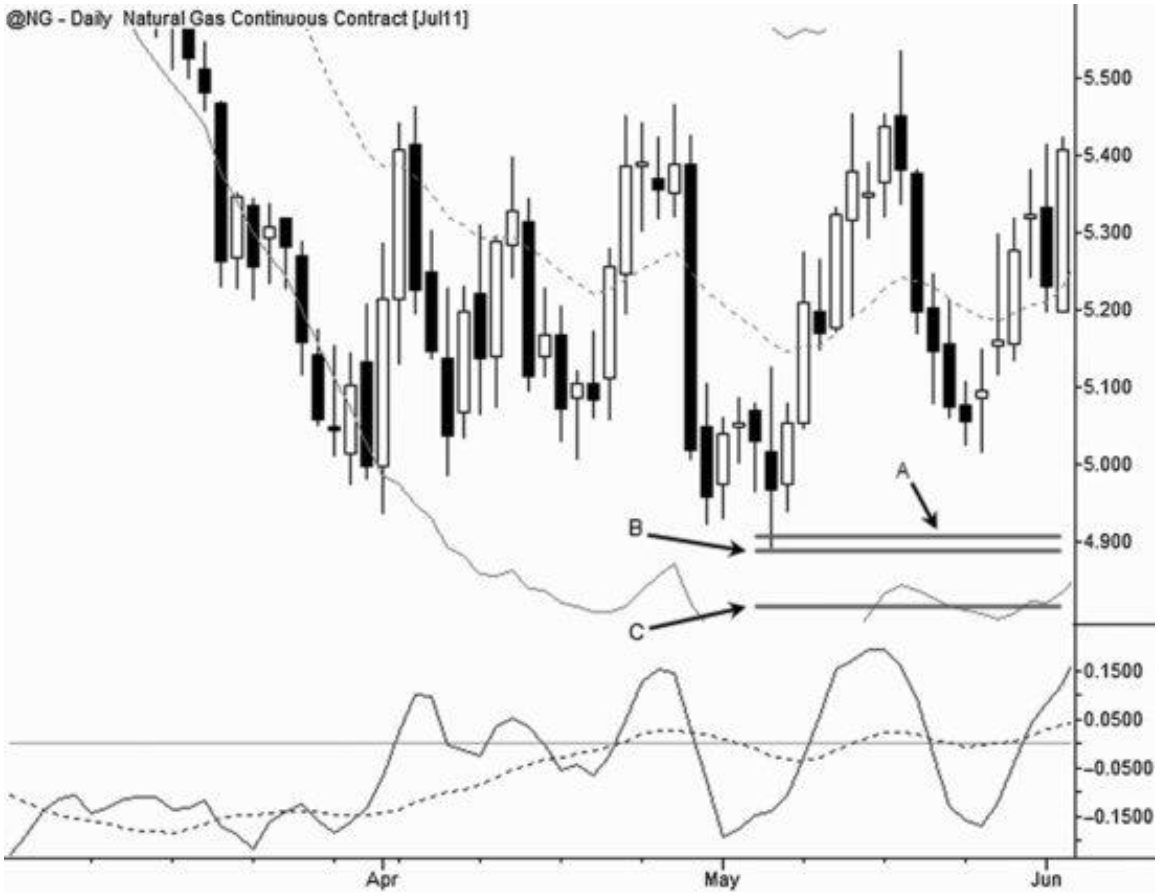
\includegraphics[width=0.5\linewidth]{support-stop-loss}
\begin{itemize}
  \item A and C are all good. A is good because it gets out before high volatility. C is a different style.
\end{itemize}
\subsubsection{Special Dangers of Clean Support/Resistance}
Many people establish large positions on other side of level, and when violated, yields great volatility.
\begin{itemize}
  \item Clean levels actually tend to set up good breakout trades beyond the level.
  \item Expect additional volatility and slippage. Your risk is probably at least twice what you think it is. In intraday trading with very tight stops, losses of 5 to 10 times your intended risk are possible.
  \item Even with these complications, it is possible to trade against these levels if you do it correctly and respect the additional risk they bring to the trade.
\end{itemize}
\subsubsection{Classic Accumulation/Distribution}
Don't pay much attention to volume. Know upthrusts and springs.

\subsubsection{Price Action around Support/Resistance}
 In other words, a large price spike down to support is likely to set up a better bounce from that level than would a slow trend down into support. In fact, a market trending down into support is not showing price rejection, and this type of pressure often presages a significant break of support. The quick spike test, or a test of an oversold market coming into support, requires real execution skills, as prices will be moving quickly, spreads will be wide, and there may be an extreme lack of liquidity in the book. In addition, there is the chance of a large loss if prices continue to drop or drop even faster. But skilled traders find that they are compensated for these risks by quick profits and a good expected value over a large set of these trades.
\subsubsection{Multiple Tests}
Each test actually weakens the level because price should not be able to return to the level if it is going to hold. Be very suspicious of levels after two tests.
\begin{itemize}
  \item What we want: As prices near the range, it violently turns the other way. If price either slowly approach the range or slowly repulsed away, not support/resistance.
  \item Price should never consolidate around a support/resistance level
\end{itemize}
\subsubsection{Trading Ranges as Funcitonal Structures}

\section{Interfaces between Trends and Ranges}
\textbf{Continuation Ranges}
\textbf{Reversal Ranges}
\textbf{Volatility Conditions in Trading Ranges}
\subsubsection{Parallel Ranges: The Box}
\subsubsection{Converging Ranges}
\subsubsection{Expanding Ranges}



\part{Trade Strategies}
\section{Failure Test}
\section{Pullback, Buying Support or Shorting Resistance}
\section{Pullback, Entering Lower Time Frame Breakout}
\section{Trading Complex Pullbacks}
\section{The Anti}
\section{Breakouts, Entering in the Preceding Base}
\section{Breakouts, Entering on the first Pullback Following}
\section{Failed Breakouts}

\part{Trade Management}
\section{Tools for Confirmation}
\subsection{MACD}
\subsubsection{Fast Line Pop}
\begin{itemize}
  \item The most important concept here is that momentum precedes price, meaning that a sharp momentum move in a market pressing to new highs will usually be followed by higher prices after a consolidation, and the reverse is true to the downside.
  \item Comparing local max/min to history:
  \begin{itemize}
    \item Use a 40-bar history as a starting point, but should be able to read the indicator without precise reference to this history very quickly.
    \item A more systematic approach could express the indicator’s value as a percentile of a look-back window, and enter retracements following an excursion into either the top or the bottom decile.
  \end{itemize}
  \item Consolidations or pullbacks following climaxes are not high-probability trades for trend continuation. Reversals or long, extended consolidations are more likely following these points.
  \begin{itemize}
    \item If an extremely large momentum move emerges that is out of all proportion to the recent history of the market, be very careful of entering retracements.
    \item In these extreme situations, the indicator will rescale so that recent history is highly compressed in a tight wiggly line. Rather than trying to read any significance into that line, accept that it shows that the market has made such an extreme move that the indicator should be disregarded.
  \end{itemize}
\end{itemize}

\subsubsection{Fast Line Divergence}
\begin{itemize}
  \item The best pullbacks are preceded by the MACD fast line making a significant new high (or low in the case of a downtrend)
  \item NOT momentum divergence $=$ new price high AND new MACD fast-line high.
  \item Momentum divergence when new price high AND MACD fast-line high equal or lower to before.
  \item Calculating momentum divergence does not require fast-line to reset at 0. Nearing 0 is good enough, can compare the two rallies even if they're part of the same rally.
  \item With this MACD, a divergence can usually be assumed to have reset or to have fulfilled its expectation when one of three conditions occurs:
  \begin{enumerate}
    \item price returns to an intermediate-term (e.g., 20-period) moving average
    \item the MACD fast line crosses the zero line from the divergent state
    \item an extended period of time (10+ bars) elapses.
  \end{enumerate}
\end{itemize}

\subsubsection{Fast Line Rule}
Don't buy when fast-line is positive, vice versa for shorting.

\subsubsection{Slow Line Rule}
If the slow line is extended above zero but the fast line pulls back below the zero line, it often makes sense to be on the lookout for long entries.
\section{Trade Management}
\section{Risk Management}
\section{Examples}

\part{Miscellaneous}
\section{The Trader's Edge}
\begin{itemize}
  \item Shifting probabilities. ie candlesticks with long tails have no predictive power, but during an accumulation can shift probabilities.
\end{itemize}
\section{The Trader's Mind}
\section{Becoming a Trader}


\end{document}
